\documentclass{article}

\usepackage{times}
\usepackage{graphicx}
\usepackage{booktabs}
\usepackage{subfigure}
\usepackage{natbib}
\usepackage{algorithm}
\usepackage{algorithmic}
\usepackage{amsmath}
\usepackage{amssymb}
\usepackage{lipsum}
\usepackage{todonotes}

\def\authnotes{1}

\newcounter{notectr}[section]
\newcommand{\thenote}{\thesubsection.\arabic{notectr}\refstepcounter{notectr}}

\newcommand{\fixme}[1]{\textcolor{red}{[FIXME: #1]}}
\newcommand{\note}[2]{$\ll$#1~\thenote: #2$\gg$}
\newcommand{\enote}[1]{\ifnum\authnotes=1 \textcolor{blue}{\note{EmilyT}{#1}}\fi}


\usepackage[accepted]{icml2017}
\icmltitlerunning{CS 287 Final Project Template}

\begin{document}

\twocolumn[
\icmltitle{A Hierarchical Recurrent Encoder-Decoder Model for Supervised Analysis of Therapeutic Alliance in Online Therapy Conversations}
\begin{icmlauthorlist}
  \icmlauthor{Emily Tseng}{}
\end{icmlauthorlist}

\vskip 0.3in
]

\begin{abstract}

As online therapy delivered via asynchronous text-chat grows more and more popular, there emerges a need for language analysis systems that can automatically infer high-level attributes of therapy conversations. Rising tension, lessening interest, and other such attributes are easily discernable to the therapist and to any human observer, but the asynchronous nature of this type of therapy means human observers are not always on hand to make such judgments. If used wisely, automated systems might assist therapists and their supervisors in preemptively flagging conversations with the patients at highest risk for abandoning treatment, and ultimately enable them to provide better care--but to achieve such systems, we need models that can capture emerging attributes of conversations as they progress.

In this work, we provide a proof of concept for a conversational forecasting model that makes use of generative pre-training to develop a neural representation of high-level conversational dynamics. Our model uses this representation to infer the patient's score for the working alliance between patient and therapist at a given point in a therapeutic conversation. Using a proprietary dataset of transcripts and patient outcomes from a major provider of online therapy, we show that this model outperforms baselines that do not use generative pretraining. Our work extends prior literature on conversational forecasting frameworks from social media exchanges to therapy conversations, which by nature have more complex long-term dependencies. We close by identifying several opportunities for next steps.

% \begin{itemize}
% \item This document describes the expected style, structure, and rough proportions for your final project write-up.
% \item While you are free to break from this structure, consider it a strong prior for our expectations of the final report.
% \item Length is a hard constraint. You are only allowed max \textbf{8 pages} in this format. While you can include supplementary material, it will not be factored into the grading process. It is your responsibility to convey the main contributions of the work in the length given.
% \end{itemize}

\end{abstract}

\section{Introduction}
\label{sec:introduction}

% Example Structure:
% \begin{itemize}
% % \item What is the problem of interest and what (high-level) are the current best methods for solving it?
% \item How do you plan to improve/understand/modify this or related methods?
% \item Preview your research process, list the contributions you made, and summarize your experimental findings.
% \end{itemize}

In therapeutic and caregiving contexts, a patient’s felt sense of \textit{alliance} with a care provider can make or break their treatment. This is particularly important in remote caregiving contexts like online therapy, where the vast majority of the connection between the patient and the caregiver takes place entirely over text-chat. As the popularity of this form of therapy grows, the therapists and supervisors who work on these platforms become akin to call-center employees: shuffling quickly between communication channels with an increasing and neverending caseload of patients demanding their immediate attention.

\fixme{todo: write out the first graf of the abstract, maybe cite Verge expose}

\fixme{add example}


In this project, we provide a proof of concept for the use of neural representations of high-level conversational dynamics in forecasting alliance between patients and therapists. We describe a model for predicting alliance at any given point in a conversation, and examine its potential using a proprietary dataset of therapy transcripts and patient-provided alliance scores from a major provider of online therapy services. We compare the performance of our model against a traditional feature-engineered method, bag-of-words, and examine variants with and without attention. Our work provides a starting point for further work on conversational forecasting in this important problem domain. To summarize, in this work we:

\begin{itemize}
  \item develop a new model extending the current state-of-the-art in conversational forecasting to meet the challenges of online therapy conversations,
  \item show our model outperforms approaches that do not make use of generative pre-training prior to the supervised task, and
  \item lay a foundation for upcoming work examining more novel approaches using a proprietary real-world dataset of text-chat therapy transcripts.
\end{itemize}

\section{Background}
\label{sec:background}

% Example Structure:
% \begin{itemize}
% \item What information does a non-expert need to know about the problem domain?
% \item What data exists for this problem?
% \item What are the challenges/opportunities inherent to the data? (High dimensional, sparse, missing data, noise, structure, discrete/continuous, etc?)
% \end{itemize}

\textbf{Online therapy data.} \fixme{What are the challenges/opportunities inherent to the data? (High dimensional, sparse, missing data, noise, structure, discrete/continuous, etc?)}


\textbf{Therapeutic alliance and WAI.} The psychology literature has had a longstanding interest in the role of the relationship between the therapist and the patient in successful psychotherapy. Early works posited that a beneficial attachment between patient and therapist enables the patient to trust the therapist enough to use his or her interpretations to bring about positive change (for a review, see Ardito \& Rabellino \citeyear{ardito2011therapeutic}). Bordin \citeyear{bordin1979generalizability} defined the concept of a \textit{working alliance} as the relational underpinning of many approaches to psychotherapy, and outlined that different types of alliance emerge from different approaches. Regardless of approach, Bordin argues, it is the \textit{strength} of the alliance that best predicts positive outcomes.

As a way to measure alliance in a given patient-therapist relationship, Horvath \& Greenberg \citeyear{horvath1989development} proposed the Working Alliance Inventory (WAI), a set of self-reported scales that measure the quality of the alliance along the three dimensions defined in Bordin's theoretical framework: (1) the \textit{bond} between patient and therapist, (2) the agreement on the \textit{goals} of the therapy, and (3) the agreement on the \textit{tasks} required to achieve those goals. Available in variants from the perspective of the patient, the therapist, and a third-party observer, the WAI has been validated as a reliable metric for alliance in several contexts (for a meta-analysis, see Martin et al. \citeyear{martin2000relation}).

\section{Related Work}
\label{sec:related-work}

\fixme{What 3-5 papers have been published in this space? How do these differ from your approach?}
\fixme{What data or methodologies do each of these works use? How do you plan to compare to these methods?}

% % Example Structure:
% \begin{itemize}
% \item What 3-5 papers have been published in this space?
% \item How do these differ from your approach?
% \item What data or methodologies do each of these works use?
% \item How do you plan to compare to these methods?
% \end{itemize}

\textbf{NLP and therapy.} \fixme{cite Althoff work, CTL papers, George paper?}

\textbf{Conversational forecasting.} Our work adapts and extends the Conversational Recurrent Architecture for ForecasTing (CRAFT), a framework integrating generative pre-training with a supervised fine-tuning model to achieve improved predictive ability on conversation-level attributes, e.g., whether an online conversation will derail into personal attacks \cite{Chang-Trouble:19}. 

Whereas CRAFT focused on prediction of a binary outcome (derailment vs. non-derailment), our work focuses on classification of progressive segments of a conversation into one of multiple outcomes (buckets of WAI scores, as described in section \ref{sec:dataset}). Chang \& Danescu-Niculescu-Mizil \citeyear{Chang-Trouble:19} also focus on social media conversations, including threads on Reddit and Wikipedia; in contrast, we study therapeutic conversations, which are longer and contain more long-range dependencies, thus presenting a more challenging modeling task.

\section{Dataset}
\label{sec:dataset}

We consider a dataset of therapy transcripts and associated patient outcomes from Talkspace, an online therapy platform. Due to the highly sensitive nature of therapy, we put significant effort into respecting patients' privacy and autonomy. All represented patients gave informed consent for the use of their data in research, and transcripts were anonymized by Talkspace before they were handed to our research team. Our study protocol was approved by our institutional IRB.

In total, our dataset consists of 5.7M messages exchanged between patients and therapists, representing 11,233 patients' full courses of treatment. 1,906 therapists are represented, with an average of 9 patients per therapist. Outcome annotations are provided in the form of patients' responses to surveys issued approximately every 3 weeks. In total, 13,742 WAI scores were provided by 6,702 patients. Patients provided an average of 2.1 WAI scores (range 1-24, stdev 2.2). 

As depicted in Figure \ref{fig:wai-distribution}, The overall distribution of scores skewed strongly towards the positive end of the spectrum (more strongly allied). Given this, in this project we formulated our predictive task as multiclass classification between three buckets of scores: 0-14, 15-19, and 20.

\begin{figure}
  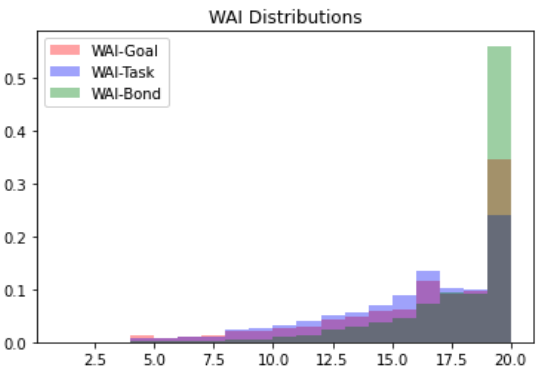
\includegraphics[width=\columnwidth]{figs/wai-distribution.png}
  \caption{Distribution of WAI scores across subdimensions.}
  \label{fig:wai-distribution}
\end{figure}


\section{Model}
\label{sec:model}

% \item What is the formal definition of your problem?
% \item What is the precise mathematical model you are using to represent it? In almost all cases this will use the probabilistic language from class, e.g.
%   \begin{equation}
%   z \sim {\cal N}(0, \sigma^2)\label{eq:1}
% \end{equation}
% But it may also be a neural network, or a non-probabilistic loss,
% \[ h_t \gets \mathrm{RNN}(x_{t}, h_{t-1} )\]

% This is also a good place to reference a diagram such as Figure~\ref{fig:diagram}.


% \begin{figure}
%   \centering
%   \missingfigure[figheight=8cm]{}
%   \caption{\label{fig:diagram} This is a good place to include a diagram showing how your model works. Examples include a graphical model or a neural network block diagram.}
% \end{figure}

Our model is an adaptation of the Conversational Recurrent Architecture for ForecasTing (CRAFT) \cite{Chang-Trouble:19}, which integrates a generative dialogue model and a supervised fine-tuning component to produce predictions utterance-by-utterance about some high-level conversational state.

\textbf{Problem definition.} We define a conversation $C$ as a variable-length sequence of $n$ utterances, $C=\{u_1,...,u_n\}$. Utterances are variable-length sequences of tokens $w$, and thus $u_n=\{w_1,...,w_{M_n}\}$, where $M_n$ is the length in tokens of utterance $n$.

Given a therapy exchange $C=\{u_1,...,u_n\}$, we generate $h^{con}_n$, a neural representation of high-level conversational state up to utterance $u_n$. We then use $h^{con}_n$ as the input to a classifier that predicts $y_n$, the label attached to the conversation up to utterance $n$. We define the label $y_n$ based on the WAI score provided by the patient at utterance $u_n$: 0 if the score is in the bucket 0-14, 1 if 15-19, and 2 if the score is 20.

\textbf{Generative component.} Following Chang et al. \citeyear{Chang-Trouble:19}, we adopted for our generative component the hierarchical recurrent encoder-decoder (HRED) architecture proposed in Sordoni et al. \citeyear{sordoni2015hierarchical} and Serban et al. \citeyear{serban2016building}. Built to model high-level conversational context, including temporal structure and dependencies between consecutive sequential inputs, HREDs are uniquely suited for conversational forecasting tasks. 

HREDs are comprised of three component recurrent neural networks (RNNs): an utterance encoder, a conversation encoder, and a decoder. First, the \textit{utterance encoder} generates for each utterance a semantic vector representation via its hidden state $h^{enc} \in \mathbb{R}^d_{enc}$, where $d_{enc}$ is the desired dimension. For each token $w_m$ in utterance $n$ of length $M$, the encoder updates its $h^{enc}$ like so:
\begin{equation}
  h^{enc}_m \gets f^{\mathrm{RNN}}_{enc}(w_{m}, h^{enc}_{m-1})
\end{equation}
The utterance encoder's hidden state at the last step, $h^{enc}_{M}$, in theory represents an embedding for the entire utterance. Following Serban et al. \citeyear{serban2016building}, $h^{enc}_{0}$ is initialized as the zero vector $\mathbf{0}$, and following Chang et al. \citeyear{Chang-Trouble:19}, we use the GRU \cite{cho2014learning} as our nonlinear gating function $f^{\mathrm{RNN}}$.

Next, the \textit{conversation encoder} uses the hidden states from each consecutive comment in a sequence of length $N$ to produce an embedding $h^{con}_n$ for the conversation up to the utterance at that point ($u_N$):
\begin{equation}
  h^{con}_n \gets f^{\mathrm{RNN}}_{con}(h^{enc}_{M_n}, h^{con}_{n-1})
\end{equation}
The conversation encoder also initializes its hidden state $h^{con}_0$ with the zero vector $\mathbf{0}$, and also uses the GRU as its nonlinearity. We denote the dimension of $h^{con}$ as $d_{con}$.

The \textit{decoder} uses the embedded conversational context $h^{con}_n$ to generate a response to utterance $n$. Following Sordoni et al. \citeyear{sordoni2015hierarchical}, it does this by first initializing its own hidden state $h^{dec} \in \mathbb{R}^{d_{dec}}$ using a nonlinear activation of $h^{con}_n$:
\begin{equation}
  h^{dec}_0 = \tanh(D h^{con}_n + b_0)
\end{equation}
Where $D \in \mathbb{R}^{d_{dec} \times d_{con}}$ projects the context embedding into decoder space, and $b_0 \in \mathbb{R}^{d_{dec}}$. 
The decoder then updates its own hidden state for each response token using the following recurrence:
\begin{equation}
  h^{dec}_{t} \gets f^{\mathrm{RNN}}_{dec}(w_{t-1}, h^{dec}_{t-1})
\end{equation}
The decoder then produces the next token in its response by producing a probability distribution over words from $h^{dec}_t$:
\begin{equation}
  w_t = f^{out}(h^{dec}_t, w_{t-1})
\end{equation}
In our implementation, following CRAFT, we supplement $f^{out}$ with attention \cite{luong2015effective}, the intuition being that certain dimensions of the context encoder states $c_t$ -- output from $f^{\mathrm{RNN}}_{con}$ alongside $h^{con}$ -- may be more informative for decoding than others. Our final $f^{out}$ is as follows:
\begin{equation}
  f^{out} = \mbox{softmax}(\tanh(W_c [h^{dec}_t|c_t]))
\end{equation}
Per Luong et al. \citeyear{luong2015effective}, we utilize the \textit{concat}-based scoring function in our global attention to compute $c_t$.

\textbf{Predictive component.} Our predictive component uses the conversational embedding up to utterance $u_n$ to generate a prediction for the WAI score at that utterance. We operationalize this as a multi-layer perceptron (MLP) that takes in the conversational state $h^{con}_n$ and produces a distribution $p(Y_n|h^{con}_n)$ over possible labels $Y=\{0,1,2\}$. Adapting from Chang et al. (\citeyear{Chang-Trouble:19}), our MLP uses three fully-connected layers and leaky ReLU activations between each layer; but for our task of multilabel classification, we use a softmax activation. The result is a model that creates a probability distribution in which each score can be interpreted as the likelihood of the given label.

We further implemented two variants of the predictive component: classifiers with and without attention \cite{luong2015effective}. The intuition here was that $h^{con}_n$ may encode many different high-level conversational attributes, not just those that have bearing on our particular outcome variable. By learning to weight some dimensions of $h^{con}_n$ above others, we may achieve better performance on targeted tasks.

\textbf{Parameters.} The parameters of our model include those used within each RNN of the generative component, $\theta_{enc}, \theta_{con}, \theta_{dec}$, as well as those used within the predictive component, $\theta_{clf}$.

Each RNN within the generative component contains a set of parameters for its constituent GRU (see Sordoni et al. \citeyear{sordoni2015hierarchical} for a longer explanation). $\theta_{dec}$ also includes parameters $D$ and $b_0$ transforming $h^{con}_n$ into $h^{dec}_0$, as well as all the parameters for \textit{concat}-scored global attention per Luong et al. \citeyear{luong2015effective}.

As for the predictive component, across both with- and without-attention variants, $\theta_{clf}$ is operationalized as a three-layer feedforward MLP. The attention variant additionally contains a layer of attention weights. 

% \fixme{What are the parameters or latent variables of this model that you plan on estimating or inferring? Be explicit. How many are there? Which are you assuming are given? How do these relate to the original problem description?}



\section{Training}
\label{sec:training}

For the generative component, training involves maximizing the log-likelihood of the provided context-reply pairs. For a given conversation $C$ comprised of $N$ utterances:
\begin{align}
  L(\theta) &= \sum^{N}_{n=1} \log(P(u_n|u_{1:n-1})) \\
  &= \sum^{N}_{n=1} \sum^{M_n}_{m=1} \log(P(w_{n,m}|w_{n,1:m-1}, u_{1:n-1}))
\end{align}

Optimization is done by applying the back-propagation through time (BPTT) algorithm standard to RNN training \cite{rumelhart1986learning}.

Similarly, training for the predictive component back-propagates the cross-entropy loss between the model output and the label. Note that when training the predictive component, we follow the principles of \textit{fine-tuning} and backpropagate through the entire model, all the way back to the encoder \cite{howard2018universal}. This nudges the embeddings learned during pretraining towards greater applicability to the predictive task.

% \begin{itemize}
% \item How do you plan on training your parameters / inferring the
%   states of your latent variables (MLE / MAP / Backprop / VI / EM / BP / ...)

% \item What are the assumptions implicit in this technique? Is it an approximation or exact? If it is an approximation what bound does it optimize?

% \item What is the explicit method / algorithm that you derive for learning these parameters?
% \end{itemize}


% \begin{algorithm}
%   \begin{algorithmic}
%     \STATE{\lipsum[1]}
%   \end{algorithmic}
%   \caption{Your Pseudocode}
% \end{algorithm}




\section{Methods}
\label{sec:methods}

\fixme{For each section: What are the exact details of the dataset that you used? (Number of data points / standard or non-standard / synthetic or real / exact form of the data)
}

\fixme{
How did you train or run inference? (Optimization method / hyperparameter settings / amount of time ran / what did you implement versus borrow / how were baselines computed).
}

\fixme{What are the exact details of the metric used?}

\textbf{Generative pre-training.} We began by training our generative model following the structure outlined in section \ref{sec:training}. From our dataset of 5.7M messages we randomly subsampled 250k pairs of contexts (sequences of utterances) and replies. Randomization allowed our model to see a variety of contexts from a variety of conversations, as opposed to repeatedly seeing subsets of the same conversations. For example, in context-reply pairs $(\{u_1,...,u_{n-1}\}, u_{n})$ and $(\{u_1,...,u_{n}\}, u_{n+1})$ from the same conversation, the subsequence of utterances $\{u_1,...,u_{n-1}\}$ repeat across both contexts.

Our generative model was implemented using Pytorch \cite{paszke2019pytorch}, and optimized using that framework's built-in Adam optimizer. Encoder and conversation encoder learning rates were set at 0.0001, and the decoder learning rate was set at 0.0005. 

\textbf{Task-specific fine-tuning.} All experiments with the predictive component of CRAFT-Multilabel initialized training with encoder, conversation encoder, and decoder parameters from the final generative model. 

\textbf{CBoW comparison.} Core to the proposed applicability of the CRAFT-Multilabel framework is its ability to represent the high-level conversational dynamics that emerge from utterances in sequence (e.g., derailment, the level of working alliance present), and make predictions about those high-level conversational dynamics by using those representations as features in a downstream task. 

To test whether our model was indeed representing higher-level semantics, we compared CRAFT-Multilabel against a cumulative bag-of-words (CBoW) model. Given a vocabulary $V$ and an input context $C_n=\{u_1,...u_n\}$, CBoW represents $C_n$ as a $|V|$-length vector of the counts of each word in $V$ in the context ($f(C_n)$). In our implementation, we normalized the raw counts of each word in $V$ according to their relative importance within their contexts, quantified by their term frequency-inverse document frequency (tf-idf). CBoW is inherently suited for online learning of progressive parts of the conversation: When faced with the next utterance in the sequence, $C_{n+1}=\{u_1,...,u_{n+1}\}$, CBoW recomputes $f(C_{n+1})$ to reflect the \textit{cumulative} word counts across the updated context.

The $|V|$-length feature vectors $f(C)$ are used as input to a simple feedforward MLP that mimics the structure of the predictive component of CRAFT-Multilabel: that is, it produces a distribution $p(Y|f(C))$ over possible labels $Y=\{0,1,2\}$. Note that the CBoW by definition only captures relative word occurrences; it does not capture word order, or even boundaries between the utterances in our contexts, to say nothing of higher-level conversational dynamics. Thus, comparison of CBoW against CRAFT-Multilabel should demonstrate the effect of incorporating such conversation-level attributes into this predictive task.

Our CBoW was an MLP trained via scikit-learn's Adam optimizer \cite{scikit-learn} for 200 iterations with a constant learning rate of 0.001. Similar to the predictive component of CRAFT-Multilabel, the MLP consisted of 2 hidden layers of size 100, each of which used a ReLU activation.

\textbf{Data.} For this proof of concept we compared \fixme{look into train vs val splits}


\section{Results}
\label{sec:results}

\fixme{add no-attn variant: What were the secondary results comparing the variants of your system?}

Table \ref{tab:results} depicts the results of our models on our held-out test sets. As shown, CRAFT-Multilabel outperforms CBoW by roughly 8 percentage points, and both outperform the naive baseline (outputting one of the three classes for every input). 

\begin{table}[t]
  \centering
  \begin{tabular}{@{}cc@{}}
  \toprule
  \textbf{Model}            & \textbf{Test-set Accuracy} \\ \midrule
  Selecting a single class           & 0.3333                           \\
  CBoW                       & 0.5577                           \\
  BERT & \\
  \textbf{CRAFT-Multilabel} & \textbf{0.6375}                  \\ \bottomrule
  \end{tabular}
  \caption{Performance of the CBoW vs. CRAFT-Multilabel models. All trials run with a test set of 159 context/label pairs evenly balanced between the 3 classes. The random baseline (a model that only outputs 1 class) is shown for comparison.}
  \label{tab:results}
\end{table}

% \begin{itemize}
% \item What were the results comparing previous work / baseline systems / your systems on the main task?
% \item What were the secondary results comparing the variants of your system?
% \item This section should be fact based and relatively dry. What happened, what was significant?
% \end{itemize}

% \begin{table*}
%   \centering
%   \missingfigure{}
%   \caption{This is usually a table. Tables with numbers are generally easier to read than graphs, so prefer when possible.}
%   \label{fig:mainres}
% \end{table*}


% \begin{table}
%   \centering
%   \missingfigure[figheight=5cm]{}
%   \caption{Secondary table or figure in results section.}
%   \label{fig:mainres}
% \end{table}


\section{Discussion}
\label{sec:discussion}

\fixme{What conclusions can you draw from the results section?}

\fixme{Is there further analysis you can do into the results of the system? Here is a good place to include visualizations, graphs, qualitative analysis of your results.}

\fixme{What questions remain open? What did you think might work, but did not?}

\begin{figure}[t]
  \centering
  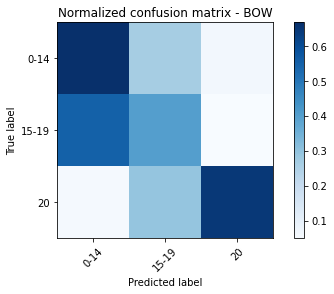
\includegraphics[width=0.9\columnwidth]{figs/cm-bow.png}
  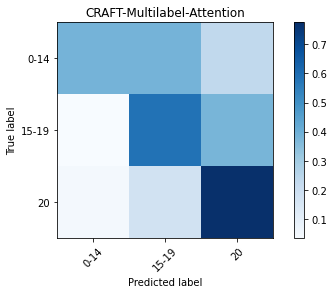
\includegraphics[width=0.9\columnwidth]{figs/cm-craftmulti.png}
  \caption{Confusion matrices for the CBoW vs. CRAFT-Multilabel models.}
  \label{fig:confusion-matrices}
\end{figure}


% \begin{figure}
%   \centering
%   \missingfigure{}
%   \missingfigure{}
%   \missingfigure{}
%   \caption{Visualizations of the internals of the system.}
% \end{figure}

\section{Conclusion}

In this work, we implemented, trained and tested a proof of concept for a model that can infer working alliance from the texts of a talk-therapy conversation. For a given segment of conversation, our model utilizes conversation-level embeddings learned via generative pre-training to forecast alliance scores across three buckets: 0-14, 15-19, and 20. Tested on a held-out sample of 159 context/label pairs, our model was shown to significantly outperform both a bag-of-words approach and a random baseline (Table \ref{tab:results}).

This proof of concept opens many avenues for next steps. 

- leverage BERT or GPT-2 embeddings
- incorporate additional features, such as timestamps
- consider variational approaches


% \section*{Acknowledgements}

% \textbf{Do not} include acknowledgements in the initial version of
% the paper submitted for blind review.

% If a paper is accepted, the final camera-ready version can (and
% probably should) include acknowledgements. In this case, please
% place such acknowledgements in an unnumbered section at the
% end of the paper. Typically, this will include thanks to reviewers
% who gave useful comments, to colleagues who contributed to the ideas,
% and to funding agencies and corporate sponsors that provided financial
% support.


\bibliography{references}
\bibliographystyle{icml2017}

\end{document}
